\chapter{THEORETICAL BACKGROUND}
\patchcmd{\chapter}{\thispagestyle{fancy}}{}{}{}
  \hrulefill\\

 
\section{Introduction To Machine Learning}
{%\noindent
Machine Learning (ML) is a subset of Artificial Intelligence that enables computers to learn from data and make decisions without being explicitly programmed. Instead of relying on predefined rules, ML systems analyze large amounts of data, identify patterns, and improve their performance over time. It plays a significant role in modern technology by automating complex tasks, increasing accuracy, and efficiently handling large-scale data. Machine Learning is generally classified into three main types: supervised learning, unsupervised learning, and reinforcement learning, each designed to solve different kinds of problems such as prediction, pattern recognition, and decision-making.}

\vspace{6pt}{%\noindent
At its core, machine learning works by training a model using historical data. The model learns patterns from this data and then applies that knowledge to new, unseen data to make predictions. The performance of a machine learning system improves as more data.}


\begin{figure}[ht]
\centering
 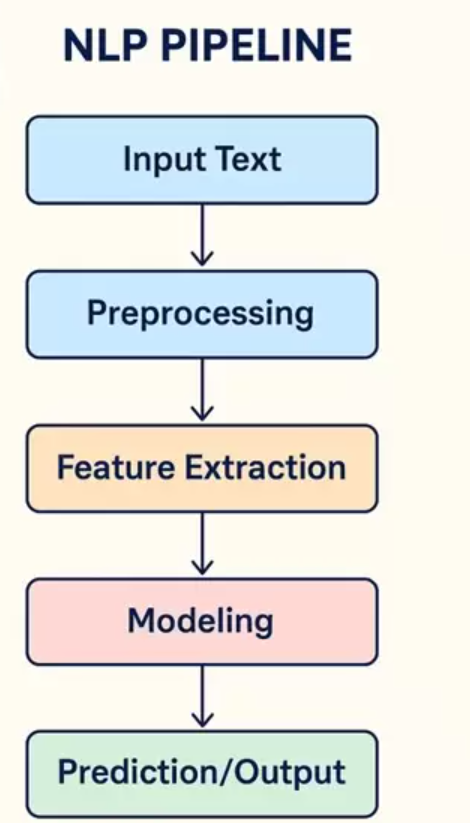
\includegraphics[width=0.4\textwidth]{images/NLP architecture.png}
 \captionof{figure}{NLP Architecture}
\end{figure}
\section{Natural Language Processing Model Pipeline}
{%\noindent
NLP models are algorithms or computational techniques used to understand, process, and generate human language. These models take textual data as input and perform tasks such as classification, translation, sentiment analysis, and information extraction. Depending on complexity, NLP models can be divided into traditional machine learning models and advanced deep learning models.}


\subsection{Input Text:}
{%\noindent
The NLP pipeline begins with input text, which is raw and unstructured data collected from various sources such as resumes, emails, documents, social media posts, or web content. This data may contain inconsistencies such as different formats, spelling variations, symbols, and irrelevant information. Since machines cannot directly understand human language, this raw input must be processed through multiple stages to extract meaningful information.}

\subsection{Preprocessing:}

Preprocessing is a critical step in the NLP pipeline where the raw text is cleaned and standardized to make it suitable for analysis. The quality of preprocessing directly affects the performance of the model.

\noindent This stage includes several sub-steps:
\begin{itemize}
\item Tokenization: Splitting text into smaller units such as words or sentences.
\item  Lowercasing: Converting all text into a uniform format (e.g., lowercase).
\item Stop-word Removal: Removing common words like “is”, “the”, “and” that do not add significant meaning.
\item Stemming and Lemmatization: Reducing words to their root or base form.
\item Removing Noise: Eliminating punctuation, special characters, numbers, and extra spaces.
\end{itemize} 
\subsection{Feature Extraction:}

After preprocessing, the text needs to be converted into a numerical representation because machine learning models cannot understand text directly. This process is called feature extraction.

\noindent Common techniques used:
\begin{itemize}
    \item Bag of Words (BoW): Represents text based on word frequency.
    \item TF-IDF: Assigns importance to words based on their frequency across documents.
    \item Word Embeddings: Converts words into dense vectors capturing semantic meaning (e.g., Word2Vec, GloVe)

This stage transforms textual data into structured data that can be fed into machine learning models.
\end{itemize}
\subsection{Modeling:}

In this stage, machine learning or deep learning models are applied to the extracted features. The model learns patterns, relationships, and structures within the data during training.

\noindent Common models include:
\begin{itemize}
    \item Machine Learning: Naive Bayes, SVM, Decision Trees.
    \item Deep Learning: RNN, LSTM, Transformer models like BERT

The choice of model depends on the complexity of the task and the dataset size. The model is trained using labeled or unlabeled data depending on the problem type.
\end{itemize}
\subsection{Prediction/Output:}

This is the final stage of the NLP pipeline where the trained model produces results based on the input data. The output can vary depending on the application.

\noindent Examples:
\begin{itemize}
    \item Classification (e.g., spam detection)
    \item Sentiment analysis (positive/negative)
    \item Resume ranking (in your project)
    \item Question generation (mock interview questions)

The output is meaningful and actionable, helping users make decisions or automate tasks.
\end{itemize}
\section{Applications}

Natural Language Processing (NLP) is widely used in various real-world applications to enable machines to understand, interpret, and generate human language. It plays a crucial role in improving interaction between humans and computers and is used across multiple domains.
\begin{figure}[ht]
\centering
 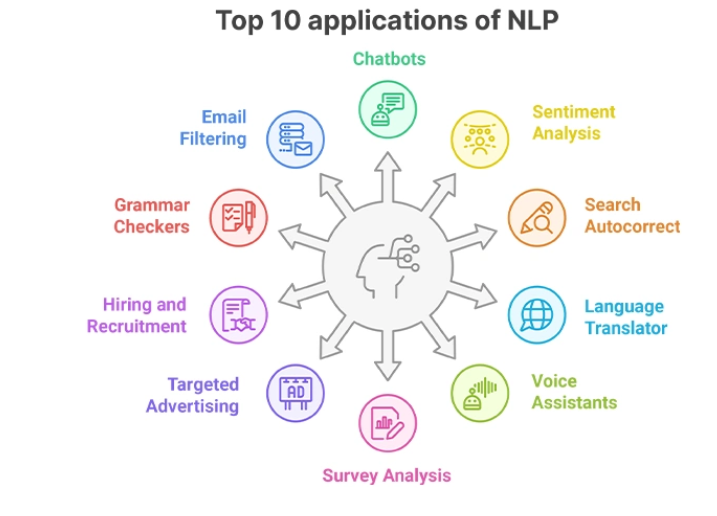
\includegraphics[width=0.6\textwidth]{images/Applications of NLP.png}
 \captionof{figure}{Applications of NLP}
\end{figure}
\subsection{Chatbots:}

Customer service and experience are the most important things for any company. It can help companies improve their products and also keep customers satisfied. But interacting with every customer manually and resolving the problems can be a tedious task. This is where Chatbots come into the picture. Chatbots help companies achieve the goal of a smooth customer experience.
\subsection{Sentiment Analysis:}

More and more people these days have started using social media to post their thoughts about a particular product, policy, or matter. These could contain some useful information about an individual’s likes and dislikes. Hence, analyzing this unstructured data can help in generating valuable insights. Natural Language Processing comes to the rescue here, too. It plays a crucial role in sentiment analysis, especially for customer data.
\subsection{Search Autocorrect and Autocomplete:}

It’s a wonderful application of natural language processing and a great example of how it is affecting millions around the world, including you and me. Search autocomplete and autocorrect both help us find accurate results more efficiently. Now, various other companies have also started using this feature on their websites, like Facebook and Quora.

\noindent The driving engine behind search-autocomplete and autocorrect is the language models. 
\subsection{Language Translator:}

Today, tools like Google Translate can easily convert text from one language to another. These tools are helping numerous people and businesses in breaking the language barrier and becoming successful.
\subsection{Voice Assistants:}

A voice assistant is a software that uses speech recognition, natural language understanding, and natural language processing to understand the verbal commands of a user and perform actions accordingly. You might say it is similar to a chatbot, but I have included voice assistants separately because they deserve a better place on this list. They are much more than a chatbot and can do many more things than a chatbot can.
\subsection{Survey Analysis:}

Surveys are an important way of evaluating a company’s performance. Companies conduct many surveys to get customers’ feedback on various products. This can be very useful in understanding the flaws and helping companies improve their products.
But the problem arises when a lot of customers take the survey, leading to an increasing data size. It becomes impossible for a person to read them all and draw a conclusion. That’s where companies use natural language processing to analyze the surveys and generate insights from them, like knowing the sentiments of users about an event from the feedback and analyzing product reviews to understand the pros and cons. Today, most companies use these methods because they provide much more accurate and useful information.



      
       
       

